\documentclass[aspectratio=169,10pt]{beamer}

\usepackage[utf8]{inputenc}
\usepackage[T5]{fontenc}
\usepackage[english,vietnamese]{babel}
\usepackage{mathptmx}
\usepackage{array}
\usepackage{booktabs}
\usepackage{graphicx}
\usepackage{tikz}
\usetikzlibrary{arrows.meta,positioning,fit,shapes.geometric}

\AtBeginDocument{\selectlanguage{vietnamese}}
\usetheme{default}
\usefonttheme{professionalfonts}
\setbeamertemplate{navigation symbols}{}
\graphicspath{{assets/}{assets/screenshots/}{assets/drawio/}}

\definecolor{EcoparkGreen}{HTML}{0F7B55}
\definecolor{EcoparkTeal}{HTML}{0891B2}
\definecolor{EcoparkAmber}{HTML}{B7791F}
\definecolor{SoftGreen}{HTML}{E8F7EF}
\definecolor{Ink}{HTML}{12201A}
\definecolor{EbpDeep}{HTML}{062E22}
\definecolor{EbpGreen}{HTML}{0F7B55}
\definecolor{EbpTeal}{HTML}{0891B2}
\definecolor{EbpAmber}{HTML}{B7791F}
\definecolor{EbpCanvas}{HTML}{F4FAF7}
\definecolor{EbpPanel}{HTML}{FFFFFF}
\definecolor{EbpBorder}{HTML}{BFDCCF}
\definecolor{EbpMuted}{HTML}{61746A}
\definecolor{EbpLogoGreen}{HTML}{25AD73}
\definecolor{EbpLogoTeal}{HTML}{0B6685}
\setbeamercolor{normal text}{fg=Ink,bg=EbpCanvas}
\setbeamercolor{structure}{fg=EbpGreen}
\setbeamercolor{frametitle}{fg=white,bg=EbpDeep}
\setbeamercolor{block title}{fg=white,bg=EbpGreen}
\setbeamercolor{block body}{fg=Ink,bg=white}
\setbeamertemplate{itemize item}{\raisebox{0.18ex}{\tikz\fill[EbpGreen] (0,0) rectangle (0.08,0.08);}}
\setbeamertemplate{itemize subitem}{\raisebox{0.22ex}{\tikz\fill[EbpTeal] (0,0) circle (0.035);}}
\setbeamertemplate{background canvas}{%
  \begin{tikzpicture}[remember picture,overlay]
    \fill[EbpCanvas] (current page.south west) rectangle (current page.north east);
    \draw[EbpBorder,opacity=0.18] (current page.south west) grid[step=0.62cm] (current page.north east);
  \end{tikzpicture}%
}
\newcommand{\EbpLogo}{%
  \tikz[baseline=-0.56ex,x=0.0156cm,y=0.0156cm]{
    \shade[rounded corners=3.5pt,left color=EbpLogoGreen,right color=EbpLogoTeal] (0,0) rectangle (46,46);
    \draw[white,opacity=0.22,line width=0.35pt,rounded corners=3.5pt] (0.55,0.55) rectangle (45.45,45.45);
    \draw[white,line width=0.9pt,line cap=round,line join=round]
      (29.5,17.5) circle (3.5);
    \draw[white,line width=0.9pt,line cap=round,line join=round]
      (16.5,17.5) circle (3.5);
    \draw[white,line width=0.9pt,line cap=round,line join=round]
      (23,17.5) -- (23,21) -- (20,24) -- (24,27) -- (26,24) -- (28,24);
    \draw[white,line width=0.9pt,line cap=round,line join=round] (26,30) circle (1);
  }%
}
\newcommand{\slidecaption}[1]{%
  \vspace{1.5mm}
  {\scriptsize\bfseries\color{EbpDeep}#1}
}
\setbeamertemplate{frametitle}{%
  \nointerlineskip
  \begin{beamercolorbox}[wd=\paperwidth,ht=0.78cm,dp=0.22cm,leftskip=0.42cm,rightskip=0.16cm]{frametitle}
    \usebeamerfont{frametitle}\bfseries\insertframetitle
    \hfill
    \raisebox{-0.18cm}{\EbpLogo}
  \end{beamercolorbox}
}
\setbeamertemplate{footline}{%
  \leavevmode%
  \hbox{%
    \begin{beamercolorbox}[wd=.74\paperwidth,ht=0.42cm,dp=0.16cm,leftskip=0.42cm]{author in head/foot}
      \scriptsize\color{EbpMuted}Ecopark Bicycle Parking Platform
    \end{beamercolorbox}%
    \begin{beamercolorbox}[wd=.26\paperwidth,ht=0.42cm,dp=0.16cm,rightskip=0.42cm plus 1fil]{date in head/foot}
      \hfill\scriptsize\color{EbpGreen}\insertframenumber/\inserttotalframenumber
    \end{beamercolorbox}%
  }%
}

\newcommand{\tightitems}{\setlength{\itemsep}{3pt}\setlength{\parskip}{0pt}}

\begin{document}

\begin{frame}[plain]
\begin{tikzpicture}[remember picture,overlay]
  \fill[EbpDeep] (current page.south west) rectangle ([xshift=0.38\paperwidth]current page.north west);
  \fill[EbpCanvas] ([xshift=0.38\paperwidth]current page.south west) rectangle (current page.north east);
  \draw[EbpBorder,line width=0.5pt] ([xshift=0.38\paperwidth]current page.south west) -- ([xshift=0.38\paperwidth]current page.north west);
  \node[anchor=north west,text=white,text width=0.30\paperwidth] at ([xshift=0.6cm,yshift=-0.55cm]current page.north west) {
    
\includegraphics[height=0.95cm]{logo-soict-hust-1.png}\\[0.42cm]
    {\scriptsize HANOI UNIVERSITY OF SCIENCE AND TECHNOLOGY}\\[0.08cm]
    {\scriptsize School of Information Communication Technology}\\[0.72cm]
    \tikz[baseline=-0.5ex]\node[rounded corners=3pt,fill=EbpGreen,text=white,inner xsep=6pt,inner ysep=2pt,font=\scriptsize\bfseries]{GCP-ready};\\[0.18cm]
    \tikz[baseline=-0.5ex]\node[rounded corners=3pt,fill=EbpTeal,text=white,inner xsep=6pt,inner ysep=2pt,font=\scriptsize\bfseries]{Mobile + desktop};\\[0.18cm]
    \tikz[baseline=-0.5ex]\node[rounded corners=3pt,fill=EbpAmber,text=white,inner xsep=6pt,inner ysep=2pt,font=\scriptsize\bfseries]{UC001--UC005};
  };
  \node[anchor=west,text width=0.52\paperwidth] at ([xshift=0.43\paperwidth,yshift=0.6cm]current page.west) {
    {\scriptsize\bfseries\color{EbpGreen}CAPSTONE PRESENTATION}\\[0.25cm]
    {\fontsize{27}{30}\selectfont\bfseries\color{Ink}Ecopark Bicycle\\Parking Platform}\\[0.2cm]
    {\large\color{EbpMuted}Thuê - trả xe đạp Ecopark trên Google Cloud Platform}\\[0.55cm]
    \begin{tabular}{@{}ll@{}}
    Kiều Sơn Tùng & 20235571 \\
    Nguyễn Phú An & 20235466 \\
    Phạm Chí Bằng & 20235477 \\
    Nguyễn Thanh Lâm & 20235519 \\
    Nguyễn Ngọc Minh & 20235533 \\
    \end{tabular}\\[0.35cm]
    {\small Supervisor: Ph.D. Bùi Thị Mai Anh \hfill Tháng 6 năm 2026}
  };
\end{tikzpicture}
\end{frame}

\begin{frame}{Mục tiêu bài toán}
\small
\begin{itemize}\tightitems
  \item Ecopark có nhiều bãi xe, nhiều loại xe và trạng thái xe thay đổi liên tục theo lượt thuê.
  \item Khách cần tìm bãi gần mình, chọn xe rảnh, gửi request và xem trạng thái yêu cầu/lượt thuê.
  \item Staff/Admin cần kiểm giấy tờ, nhận cọc 200k, giao xe, nhận trả xe khác bãi và xuất vé.
  \item Quản lý cần dashboard doanh thu, trạng thái đội xe, audit log và CSV report theo bộ lọc.
  \item Nhóm triển khai một platform web có UI desktop/mobile và target deploy lên GCP.
\end{itemize}
\end{frame}

\begin{frame}{Actor Và Use Case}
\centering
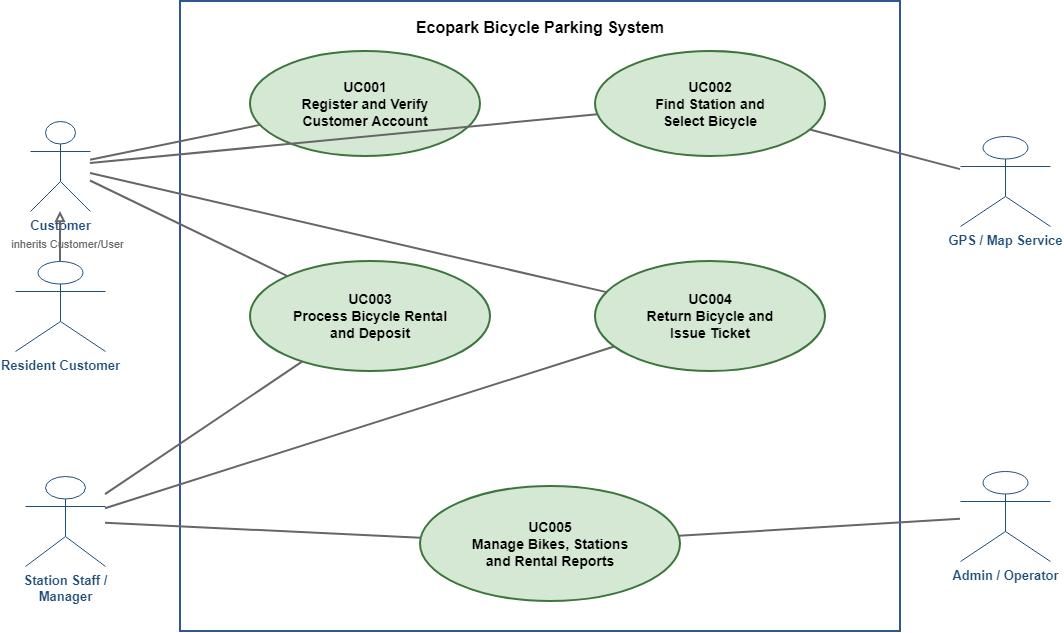
\includegraphics[width=\textwidth,height=0.82\textheight,keepaspectratio]{uc_overview.png}
\end{frame}

\begin{frame}{Scope Đã Implement Theo UC001--UC005}
\scriptsize
\begin{tabular}{p{0.12\textwidth}p{0.31\textwidth}p{0.47\textwidth}}
\toprule
\textbf{UC} & \textbf{Mục tiêu} & \textbf{Kết quả trong platform} \\
\midrule
UC001 & Tài khoản và xác thực khách & Đăng ký/đăng nhập, validation họ tên, phone, CCCD/CMND, resident discount. \\
UC002 & Tìm bãi và chọn xe & GPS demo/vị trí nhập tay, range filter, bike type filter, chọn xe rảnh, gửi/hủy request. \\
UC003 & Giao xe và đặt cọc & Staff xác nhận giấy tờ, cọc 200k, giấy tờ giữ lại và chuyển xe sang rented. \\
UC004 & Trả xe và xuất vé & Trả khác bãi, tính phí, giảm cư dân, phụ thu trễ, condition note và ticket summary. \\
UC005 & Quản lý vận hành & CRUD bãi/xe, status reason, report charts, audit log, CSV export. \\
\bottomrule
\end{tabular}
\end{frame}

\begin{frame}{Kiến Trúc GCP}
\centering
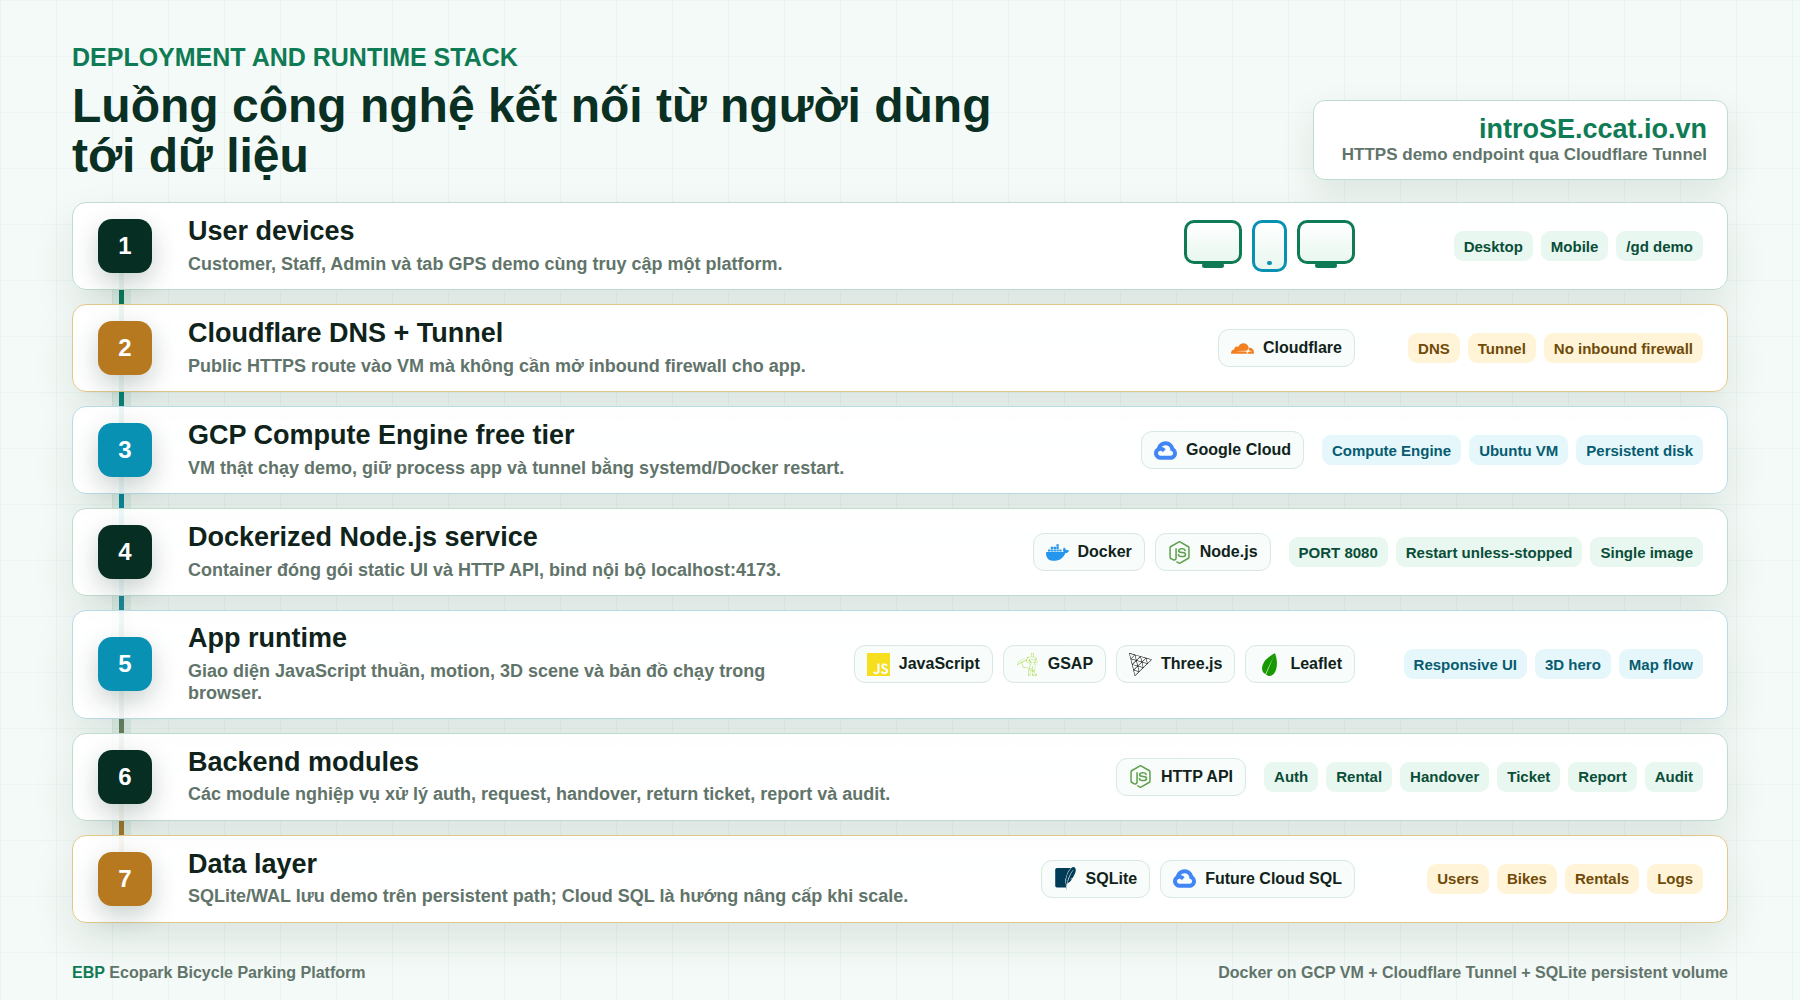
\includegraphics[width=\textwidth,height=0.86\textheight,keepaspectratio]{techstack/tech_stack_architecture.png}
\end{frame}

\begin{frame}{Thiết Kế Dữ Liệu}
\centering
\resizebox{0.96\textwidth}{!}{%
\begin{tikzpicture}[
  domaincard/.style={draw=EbpGreen,thick,rounded corners=4pt,fill=SoftGreen,minimum width=3.25cm,minimum height=1.78cm,align=left,font=\scriptsize,inner sep=7pt},
  core/.style={draw=EbpTeal,very thick,rounded corners=4pt,fill=cyan!8,minimum width=3.55cm,minimum height=2.12cm,align=left,font=\scriptsize,inner sep=8pt},
  support/.style={draw=EbpAmber,thick,rounded corners=4pt,fill=yellow!10,minimum width=3.25cm,minimum height=1.48cm,align=left,font=\scriptsize,inner sep=7pt},
  arr/.style={-{Latex[length=2mm]},draw=Ink,line width=0.85pt}
]
\node[core] (rental) at (0,0) {
  \textbf{Giao dịch thuê - trả}\\[1mm]
  RENTAL\_REQUESTS\\
  RENTALS\\
  DEPOSITS\\
  TICKETS
};
\node[domaincard] (identity) at (-4.55,0) {
  \textbf{Người dùng \& hồ sơ}\\[1mm]
  USERS\\
  CUSTOMER\_PROFILES\\
  RESIDENT\_CARDS\\
  STAFF
};
\node[domaincard] (fleet) at (4.55,0) {
  \textbf{Bãi \& đội xe}\\[1mm]
  STATIONS\\
  BIKE\_TYPES\\
  BIKES\\
  BIKE\_STATUS\_LOGS
};
\node[support] (policy) at (0,2.35) {
  \textbf{Chính sách phí}\\
  resident discount, late surcharge, deposit
};
\node[support] (ops) at (0,-2.35) {
  \textbf{Báo cáo vận hành}\\
  revenue, fleet status, audit trail
};
\draw[arr] (identity.east) -- (rental.west);
\draw[arr] (fleet.west) -- (rental.east);
\draw[arr] (policy.south) -- (rental.north);
\draw[arr] (rental.south) -- (ops.north);
\end{tikzpicture}
}
\vspace{0.2cm}
\small ERD chi tiết nằm trong report; slide này chỉ giữ các quan hệ dữ liệu chính quanh lõi thuê - trả.
\end{frame}

\begin{frame}{Vòng Đời Thuê Xe}
\centering
\resizebox{0.92\textwidth}{!}{%
\begin{tikzpicture}[
  state/.style={draw=EcoparkGreen,thick,rounded corners=2pt,fill=SoftGreen,minimum width=2.9cm,minimum height=0.92cm,align=center,font=\scriptsize},
  bad/.style={draw=EcoparkAmber,thick,rounded corners=2pt,fill=yellow!12,minimum width=2.9cm,minimum height=0.92cm,align=center,font=\scriptsize},
  arr/.style={-{Latex[length=2.2mm]},thick,draw=Ink}
]
\node[state] (available) {Bike available};
\node[state,right=0.95cm of available] (pending) {Request\\pending pickup};
\node[state,right=0.95cm of pending] (rented) {Rental\\in progress};
\node[state,right=0.95cm of rented] (ticket) {Ticket\\completed};
\node[bad,below=0.85cm of pending] (cancel) {Cancel / expired};
\node[bad,below=0.85cm of ticket] (broken) {Broken / review};
\draw[arr] (available) -- (pending);
\draw[arr] (pending) -- (rented);
\draw[arr] (rented) -- (ticket);
\draw[arr] (pending) -- (cancel);
\draw[arr] (cancel) -| (available);
\draw[arr] (ticket) -- (broken);
\end{tikzpicture}
}
\end{frame}

\begin{frame}{Customer Mobile Flow}
\begin{columns}[T,totalwidth=0.98\textwidth]
\begin{column}{0.31\textwidth}
\centering
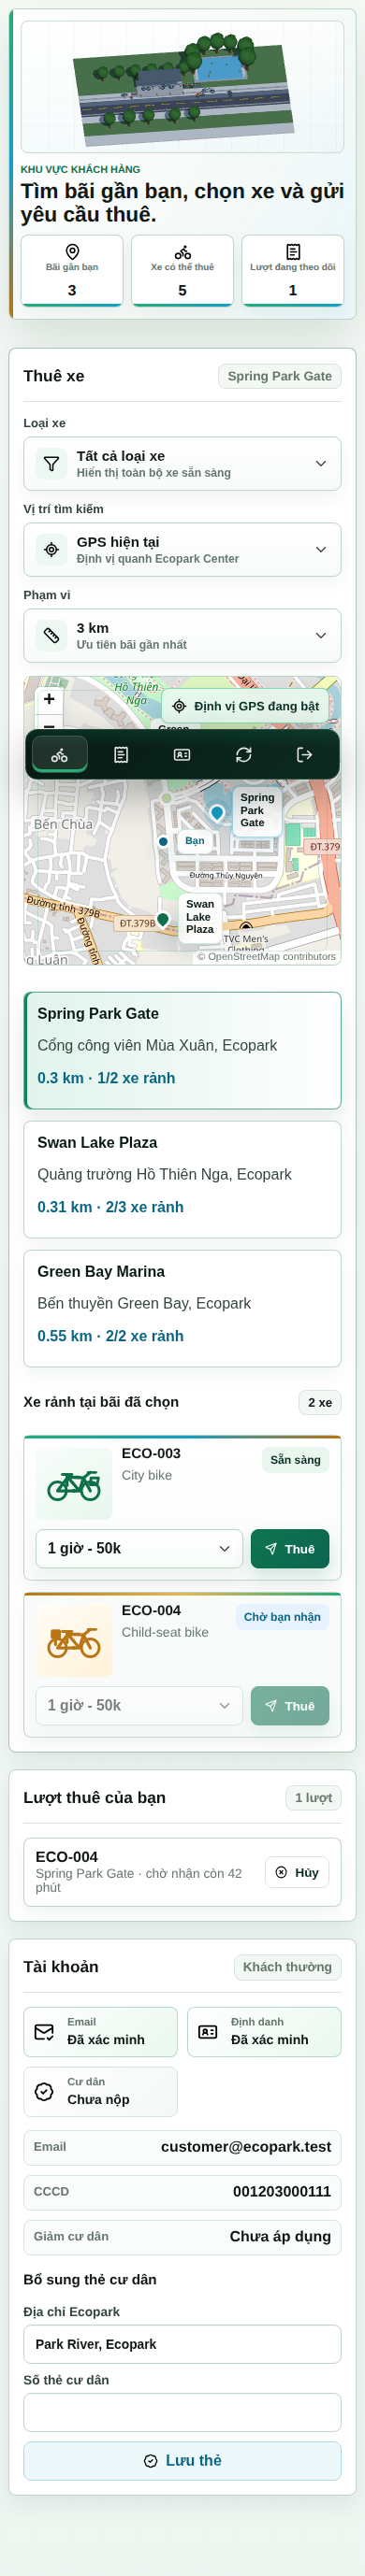
\includegraphics[width=\linewidth,height=0.62\textheight,keepaspectratio,trim=0 2030bp 0 0,clip]{customer_mobile.png}
\slidecaption{Tổng quan}
\end{column}
\begin{column}{0.31\textwidth}
\centering
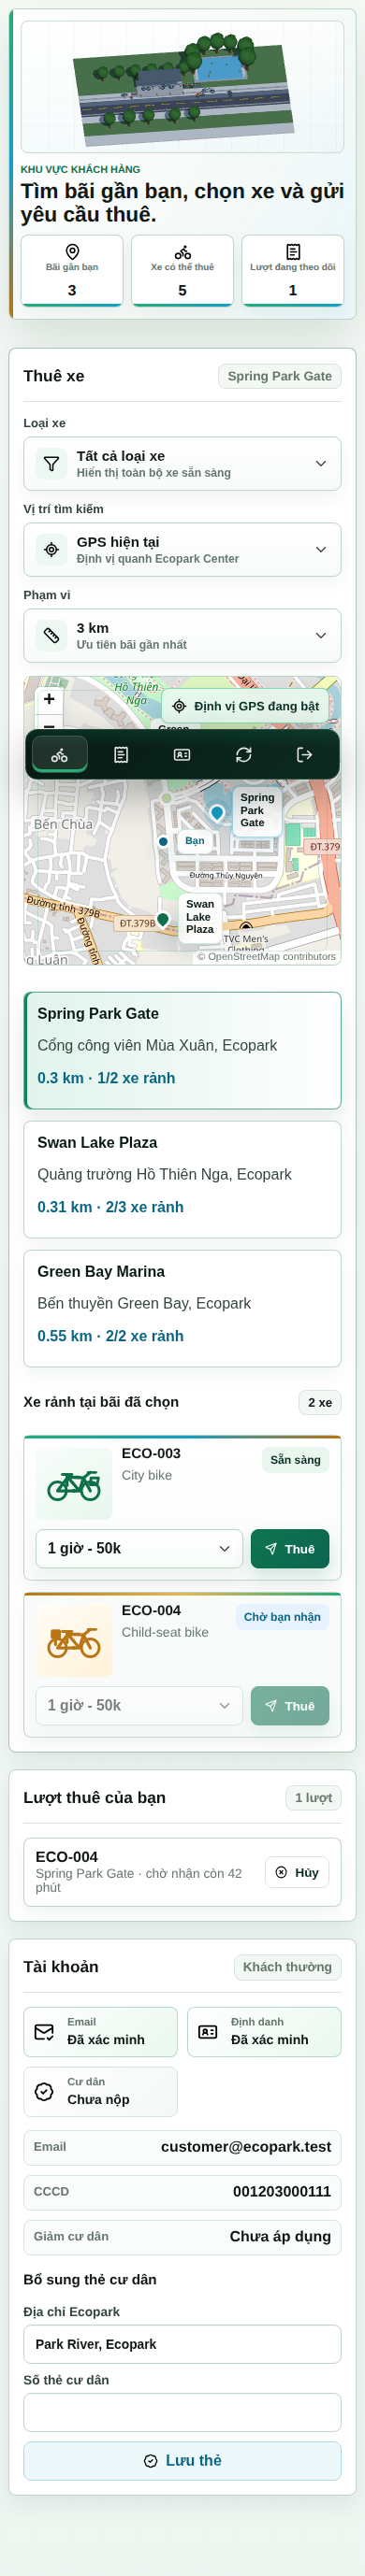
\includegraphics[width=\linewidth,height=0.62\textheight,keepaspectratio,trim=0 1216bp 0 880bp,clip]{customer_mobile.png}
\slidecaption{Tìm bãi}
\end{column}
\begin{column}{0.31\textwidth}
\centering
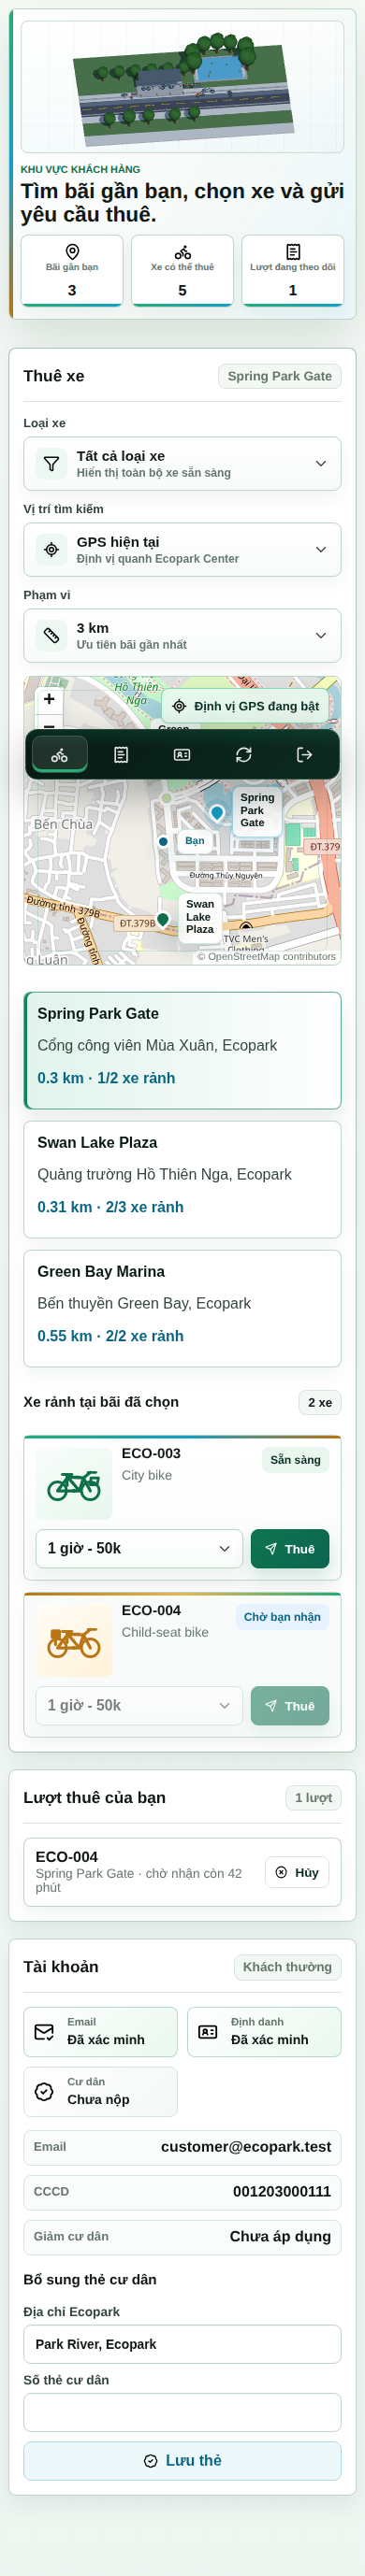
\includegraphics[width=\linewidth,height=0.62\textheight,keepaspectratio,trim=0 600bp 0 1450bp,clip]{customer_mobile.png}
\slidecaption{Chọn xe}
\end{column}
\end{columns}
\vspace{0.15cm}
\scriptsize Flow mobile được tách thành các lát không cắt qua bottom dock: tổng quan, kết quả bãi gần nhất và chọn xe rảnh.
\end{frame}

\begin{frame}{Operations UI}
\begin{columns}[T,totalwidth=0.98\textwidth]
\begin{column}{0.49\textwidth}
\centering
\begin{minipage}[t][0.72\textheight][c]{\linewidth}
\centering

\includegraphics[width=\linewidth,height=0.70\textheight,keepaspectratio,trim=0 2450bp 0 0,clip]{operations_desktop.png}
\end{minipage}
\end{column}
\begin{column}{0.49\textwidth}
\centering
\begin{minipage}[t][0.72\textheight][c]{\linewidth}
\centering

\includegraphics[width=\linewidth,height=0.70\textheight,keepaspectratio,trim=0 1300bp 0 1020bp,clip]{operations_desktop.png}
\end{minipage}
\end{column}
\end{columns}
\vspace{-1mm}
\begin{columns}[T,totalwidth=0.98\textwidth]
\begin{column}{0.49\textwidth}
\centering
\slidecaption{Tổng quan vận hành}
\end{column}
\begin{column}{0.49\textwidth}
\centering
\slidecaption{Báo cáo, yêu cầu và pipeline trả xe}
\end{column}
\end{columns}
\vspace{0.15cm}
\scriptsize Screenshot operations được chia thành hai lát để giữ dashboard, biểu đồ và khu vực xử lý đủ lớn khi thuyết trình.
\end{frame}

\begin{frame}{Light/Dark Mode}
\begin{columns}[T,totalwidth=0.98\textwidth]
\begin{column}{0.58\textwidth}
\centering
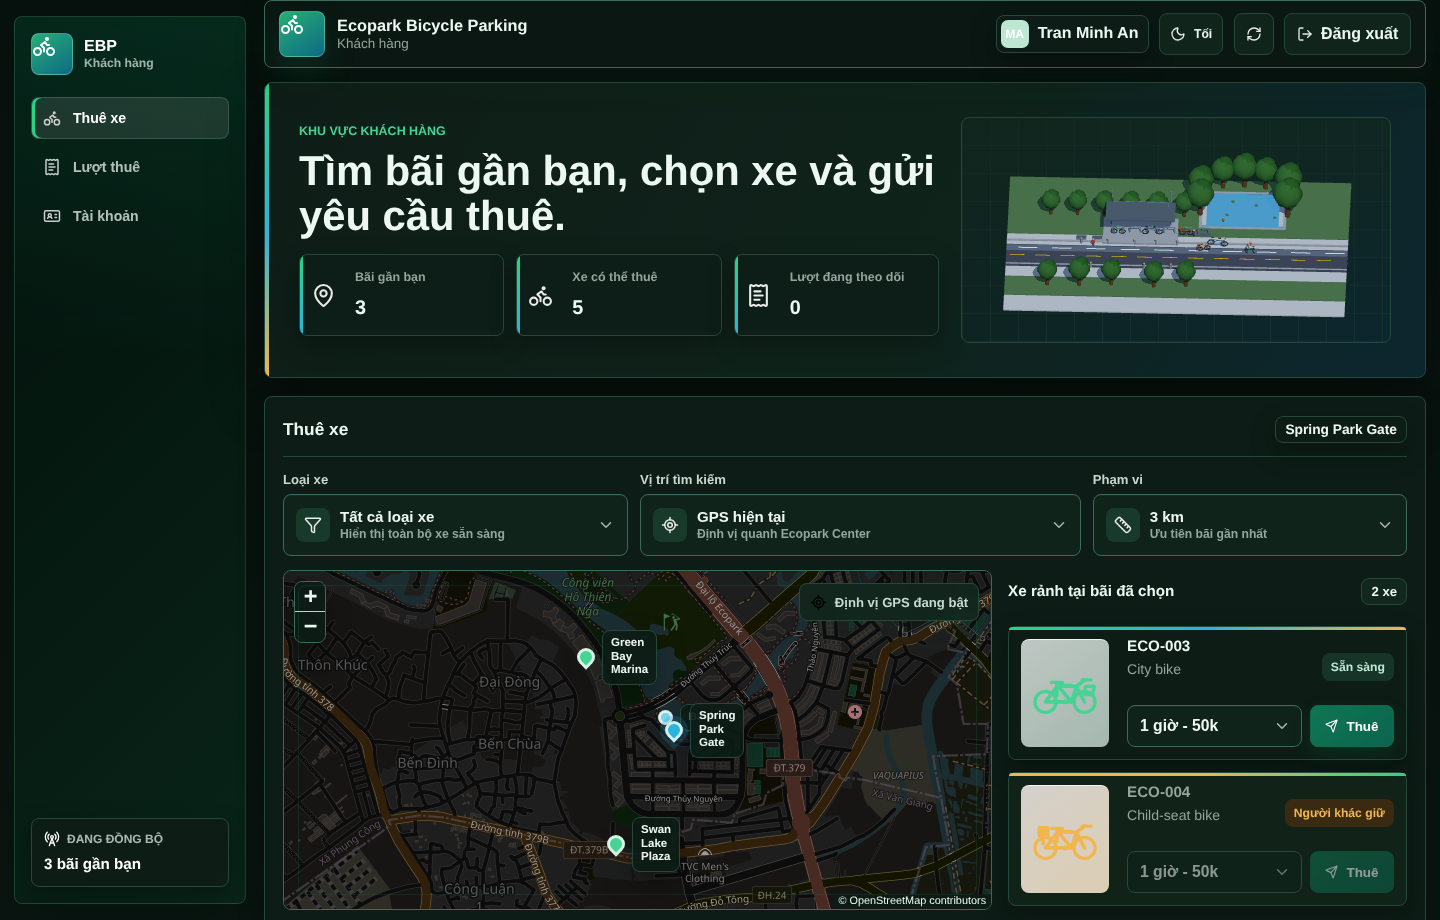
\includegraphics[width=\linewidth,height=0.72\textheight,keepaspectratio]{darkmode_customer.png}
\end{column}
\begin{column}{0.37\textwidth}
\small
\begin{itemize}\tightitems
  \item Theme \textit{Sáng}, \textit{Tối}, \textit{Hệ thống} lưu trong trình duyệt.
  \item Leaflet map có dark treatment riêng, không còn mảng bản đồ trắng gắt.
  \item Card tài khoản, dropdown, chart và form dùng cùng design tokens.
  \item Scene 3D vẫn giữ tương phản để nhìn rõ xe, đường, hồ và cây.
\end{itemize}
\end{column}
\end{columns}
\end{frame}

\begin{frame}{Demo Director Cho Alternative Flow}
\begin{columns}[T,totalwidth=0.98\textwidth]
\begin{column}{0.61\textwidth}
\centering

\includegraphics[width=\linewidth,height=0.72\textheight,keepaspectratio]{gps_demo.png}
\end{column}
\begin{column}{0.34\textwidth}
\scriptsize
\begin{tikzpicture}[
  stepcard/.style={draw=EbpBorder,rounded corners=3pt,fill=white,text width=0.95\linewidth,minimum height=1.05cm,align=left,inner sep=6pt}
]
\node[stepcard] at (0,0) {\textbf{1. Chọn session}\\Customer đang request hoặc đang thuê.};
\node[stepcard] at (0,-1.35) {\textbf{2. Kéo GPS người dùng}\\Di chuyển theo polyline đường, không nhảy qua hồ/nhà.};
\node[stepcard] at (0,-2.70) {\textbf{3. Tua giờ hệ thống}\\Dùng để demo quá hạn và phụ thu trễ.};
\node[stepcard] at (0,-4.05) {\textbf{4. Kiểm geofence}\\Nhận/trả xe chỉ hợp lệ khi ở gần bãi.};
\end{tikzpicture}
\end{column}
\end{columns}
\end{frame}

\begin{frame}{API Và Backend Implementation}
\scriptsize
\begin{tabular}{p{0.24\textwidth}p{0.20\textwidth}p{0.46\textwidth}}
\toprule
\textbf{Nhóm API} & \textbf{Role} & \textbf{Endpoint chính} \\
\midrule
Auth/Profile & Public/Customer & \texttt{/api/auth/register}, \texttt{/api/auth/login}, \texttt{/api/customer/resident-card}. \\
Station/Bike & Customer & \texttt{/api/stations}, \texttt{/api/stations/:id/bikes}, \texttt{/api/rental-requests}. \\
Handover/Return & Staff/Admin & \texttt{/api/staff/pending-requests}, \texttt{/api/staff/handover}, \texttt{/api/staff/return}. \\
Admin/Report & Staff/Admin & \texttt{/api/admin/bikes}, \texttt{/api/admin/reports}, \texttt{/api/admin/bike-status-logs}. \\
\bottomrule
\end{tabular}
\vspace{0.25cm}
\begin{itemize}\tightitems
  \item Server-side validation cho họ tên, phone, CCCD/CMND và dữ liệu trùng.
  \item Rental/handover/return chạy qua transaction để tránh double-booking.
  \item Audit log lưu thay đổi trạng thái xe cùng người đổi, bãi và lý do.
\end{itemize}
\end{frame}

\begin{frame}{Dashboard Báo Cáo}
\begin{columns}[T,totalwidth=0.98\textwidth]
\begin{column}{0.58\textwidth}
\centering

\includegraphics[width=\linewidth,height=0.72\textheight,keepaspectratio,trim=240bp 2550bp 0 430bp,clip]{operations_desktop.png}
\end{column}
\begin{column}{0.37\textwidth}
\small
\begin{itemize}\tightitems
  \item Doanh thu theo kỳ dùng cùng scale tiền giữa các chart.
  \item Fleet status cho biết xe sẵn sàng, đang thuê, cần sửa.
  \item Lượt thuê và phụ thu trễ hiển thị cạnh bảng report gốc.
  \item CSV export dùng đúng filter đang chọn trên dashboard.
  \item Audit log giúp truy vết ai đổi trạng thái xe và vì sao.
\end{itemize}
\end{column}
\end{columns}
\end{frame}

\begin{frame}{Testing Và Evidence}
\small
\begin{tikzpicture}[
  card/.style={draw=EbpBorder,rounded corners=3pt,fill=white,text width=4.85cm,minimum width=5.35cm,minimum height=1.52cm,align=left,inner xsep=9pt,inner ysep=8pt},
  badge/.style={font=\Large\bfseries,text=EbpGreen},
  label/.style={font=\scriptsize\bfseries,text=Ink},
  note/.style={font=\scriptsize,text=EbpMuted}
]
\node[card] (api) at (0,1.58) {
  \begin{minipage}{4.42cm}\raggedright
  {\Large\bfseries\color{EbpGreen}21/21}\\[0.45mm]
  {\scriptsize\bfseries Backend API tests}\\[0.25mm]
  {\scriptsize Geofence, handover, ticket, report, audit}
  \end{minipage}
};
\node[card] (ui) at (6.0,1.58) {
  \begin{minipage}{4.42cm}\raggedright
  {\Large\bfseries\color{EbpTeal}4 viewports}\\[0.45mm]
  {\scriptsize\bfseries UI smoke}\\[0.25mm]
  {\scriptsize Desktop, staff-wide, medium, mobile}
  \end{minipage}
};
\node[card] (uc) at (0,-0.72) {
  \begin{minipage}{4.42cm}\raggedright
  {\Large\bfseries\color{EbpAmber}UC smoke}\\[0.45mm]
  {\scriptsize\bfseries End-to-end demo path}\\[0.25mm]
  {\scriptsize /gd, request/cancel, handover, return, CSV}
  \end{minipage}
};
\node[card] (ci) at (6.0,-0.72) {
  \begin{minipage}{4.42cm}\raggedright
  {\Large\bfseries\color{EbpGreen}CI/CD}\\[0.45mm]
  {\scriptsize\bfseries GitHub Actions}\\[0.25mm]
  {\scriptsize node --check, coverage, smoke, Docker}
  \end{minipage}
};
\end{tikzpicture}
\vspace{0.26cm}
\begin{center}
\begin{tikzpicture}
\node[draw=EbpBorder,rounded corners=3pt,fill=SoftGreen,text width=0.88\textwidth,inner sep=7pt,align=left] {
  \scriptsize\textbf{Điểm nổi bật:} UC smoke đi qua đúng luồng demo: customer gửi request, staff giao xe, customer xác nhận bãi trả trong geofence, staff xuất vé, dashboard cập nhật chart và audit log.
};
\end{tikzpicture}
\end{center}
\end{frame}

\begin{frame}{Mở Demo Trực Tiếp}
\begin{columns}[T,totalwidth=0.96\textwidth]
\begin{column}{0.52\textwidth}
\centering

\includegraphics[width=\linewidth,height=0.68\textheight,keepaspectratio]{gps_demo.png}
\end{column}
\begin{column}{0.42\textwidth}
\small
\begin{enumerate}\tightitems
  \item Mở Customer, Staff/Admin và tab \texttt{/gd}.
  \item Kéo GPS người dùng vào bán kính bãi nhận, gửi request.
  \item Staff đối chiếu giấy tờ, nhận cọc 200k và giao xe.
  \item Customer xác nhận bãi trả; Staff xuất vé và xem phụ thu.
  \item Chốt bằng dashboard, audit log và CSV export.
\end{enumerate}
\vspace{0.2cm}
{\scriptsize\bfseries\color{EbpGreen}Demo live: chạy 5 bước trên app.}
\end{column}
\end{columns}
\end{frame}

\end{document}
